% LaTeX template for thesis and dissertation ETDs
%
% Created by:
% Benjamin Hilburn
% bhilburn@vt.edu 
%
% The formatting guidelines that appear in this template are based on the ETD 
% guidelines, avaliable here: http://etd.vt.edu/stdformat.html
%
% This file is based on the original ETD template, created by:
% Neill Kipp, nkipp@vt.edu, September 6, 1997
% 
% If you check out the entire source tree of this ETD example, including the 
% images/ and refs/ subdirectory, you can compile this document and produce an 
example PDF ETD using the instructions below:

% Usage:
% This template provides for an abbreviation list, and bibliography. In order to 
% use these features, you must have bibtex installed with your LaTeX suite, and 
% run additional commands during compilation time.  Assuming that your source 
% file is called 'etd_template.tex', and you wished to produce a PDF output 
% using the pdflatex compiler, the commands would be:
%
% $ pdflatex etd_template.tex
% $ pdflatex etd_template.tex
% $ bibtex etd_template
% $ makeindex etd_template.nlo -s nomencl.ist -o etd_template.nls
% $ pdflatex etd_template.tex
% $ pdflatex etd_template.tex
%
% Note that running the LaTeX compiler twice, at the end is necessary. The first 
% run produces a list of references to elements in the document (tables, 
% figures, sections, etc.,), but can't link to the references without first 
% compiling the whole document. You can then re-compile, and the compiler will 
% properly link the document references and references themselves.  The first 
% two commands in the series, which also run the compiler twice, produce the 
% files necessary to create the bibliography and abbreviation index.


% The 'report' class will default to a single-sided, portrait document with a  
% title page and chapter-based layout.
\documentclass[pdftex,12pt,onecolumn]{report}

% These commands define the default whitespace measurements, as specified by 
% ETD guidelines. 
\setlength{\textwidth}{6.5in}
\setlength{\textheight}{8.5in}
\setlength{\evensidemargin}{0in}
\setlength{\oddsidemargin}{0in}
\setlength{\topmargin}{0in}
\setlength{\parindent}{0pt}
\setlength{\parskip}{0.1in}

% The default formatting for thesis pages should be double-spaced, although we 
% need to allow for single-space sections (such as the abstract page). This 
% package allows us to modify the spacing on a per-block basis, and setting the 
% baselinestretch to {2} makes the default formatting double-spaced.
\usepackage{setspace}
\renewcommand{\baselinestretch}{2}

% LaTeX provides for many font options. Feel free to experiment with them, and 
% choose one that you like best.  The ETD specifies fonts in the sytle of Times, 
% Courier, or Helvetica.  The Palatino font package is kind of a mix of Times 
% and Helvetica, and is my personal favorite of the default font packages.
\usepackage{palatino}
\fontsize{12}{14}

% These packages define how images are used and rendered in your thesis.  You 
% should leave the top three alone, and only modify the graphicspath and 
% GraphicsExtension options.  Note that LaTeX cannot use all types of graphics, 
% so double check that graphicx supports your graphics extension if it is 
% anything other than a pdf, jpeg, or png before attempting to add it to the 
% list. The graphicspath is exactly what it sounds like - a list of directories 
% where images used in your thesis are. In the example below, there is a 
% sub-directory of the current directory called 'images' where the image files 
% are.
\usepackage[pdftex]{graphicx}
\usepackage[center]{caption}
\usepackage{float}
\graphicspath{{./images/}}
\DeclareGraphicsExtensions{.pdf,.jpeg,.png}

% By default, LaTeX tables must appear on a single page.  This can sometimes 
% create problems, where the bottom portion of a long table will simply get 
% truncated.  This package allows for multi-page tables.  An example of such a 
% table appears in the body of this document.
\usepackage{longtable}

% Re-define the arraystretch command, which controls the whitespace in a row of 
% a table.  By setting it to be a little taller than single-space, it keeps the 
% row lines off of the text, which is a rather annoying artifact.
\renewcommand{\arraystretch}{1.5}

% Use advanced math packages for algorithm rendering. There are numerous 
% examples regarding how to use these packagas online.  They are pretty much 
% standard, now, in terms of equation-rendering.
\usepackage[cmex10]{amsmath}
\usepackage{algorithmic}

% These packages define alignment options for lists, mathematical expressions, 
% and tables.  They provide additional commands you can use to fine-tune the 
% appearance of these elements, although the defaults provided are generally 
% pretty good. 
\usepackage{array}
\usepackage{mdwmath}
\usepackage{mdwtab}

% The subfigure package allows you to have figures that consist of multiple 
% sub-figures(e.g., Figure 1.2(a), (b), and (c).
\usepackage[font=footnotesize]{subfig}

% If you notice that some words are being hyphenated in awkward places by LaTeX,  
% you can specify where in the word the split will occur.
\hyphenation{Config-uration Archi-tecture}

% This package tells LaTeX how to create a list of abbreviations at the start of 
% your document.  In order to add an acronym to this 
% list, you must do it manually.  This can be done with the 'nomenclature 
% command', which is used like so:
% \nomenclature{NSF}{National Science Foundation}
% Acronym definitions can appear anywhere in the body of your work (i.e., after 
% the \begin{document} command. 
\usepackage{nomencl}
\makenomenclature

% This command sets the name of the abbreviation list when it is printed in the 
% document. 
\renewcommand{\nomname}{List of Abbreviations}

% This package turns URLs in your document into clickable-URLs. This is 
% especially useful for references.
\usepackage{url}

% PDFs have a lot of available meta-data in them, including fields that define 
% how the document appears when it is opened in a reader.  Additionally, LaTeX 
% can create hyperlinks in your document, such that clicking on something in 
% Table of Contents, or clicking on a label, takes you to that item in the 
% document. The below fields define this functionality. If you don't want this 
% functionaliy, simply delete the below package options.
\usepackage[breaklinks]{hyperref}
\hypersetup{
    bookmarks=true,							% show bookmarks bar?
    unicode=true,         					% non-Latin characters
    pdftoolbar=true,							% show Acrobat�s toolbar?
    pdfmenubar=false,						% show Acrobat�s menu?
    pdffitwindow=false,						% window fit to page when opened
    pdftitle={The Title of Your Thesis},					% title
    pdfauthor={Jane A. Doe},									% author
    pdfsubject={M.S. Thesis of Hacker Engineering},	% subject
    pdfcreator={Jane A. Doe},				% creator of the document
    pdfnewwindow=true,						% links in new window
    colorlinks=false,						% false: boxed links; true: colored links
}
\urlstyle{same}

\begin{document}

% This defines your title page.  The ETD is very specific about how this page is 
% formatted, and your ETD submission will likely be rejected if any of the below 
% formatting is changed.  Also, note that the ETD requires that all committee 
% members have First, Middle Initial, and Last names, and no titles (the names 
% MUST NOT have Dr. in front of them, or Ph.D after them). In this example, one 
% committee member lacks a middle initial.  If one of your committee members 
% insists on not using a middle initial, you will simply have to explain this to 
% your reviewer, and it should get accepted with that caveat.
\thispagestyle{empty}
\pagenumbering{roman}
\begin{center}
{\Large 
The Title of Your Thesis
}
\vfill
Jane A. Doe
\vfill
Thesis submitted to the Faculty of the \\
Virginia Polytechnic Institute and State University \\
in partial fulfillment of the requirements for the degree of
\vfill
Master of Science \\
in \\
Hacker Engineering
\vfill
Albert Einstein, Chair \\
Claude E. Shannon \\
Carl E. Sagan
\vfill
April 22nd, 2011 \\
Blacksburg, Virginia
\vfill
Keywords: buzzword, slightly older buzzword, buzzword you made up, unrelated topic buzzword
\\
Copyright 2011, Jane A. Doe
\end{center}
\pagebreak


% The following defines your abstract page.  The abstract page is special in 
% that it ignores most of the formatting guidelines that exist in the rest of 
% your document.  Pay careful attention to the formatting procedure specified 
% below.
\thispagestyle{empty}
\begin{singlespace}
\begin{center}
{\large The Title of Your Thesis}
\vfill
Jane A. Doe
\vfill
ABSTRACT
\vfill
\end{center}
Note that the ETD restricts thesis abstricts to 250 words, and dissertation 
abstracts to 350 words. Whether or not this is enforced depends on your 
particular ETD reviewer.

Lorem ipsum dolor sit amet, consectetur adipiscing elit. Nulla vestibulum
tristique augue, in bibendum dui vestibulum vitae. Pellentesque in sapien eu
arcu fringilla aliquet. Praesent volutpat vulputate ante eu rutrum. Quisque 
pellentesque molestie diam at lobortis. Phasellus nec turpis est, vitae volutpat 
lectus. Mauris id enim sit amet quam dictum iaculis quis nec quam. Pellentesque
quis ultricies felis. Donec venenatis viverra lobortis. Proin accumsan dolor nec
est blandit lobortis. Suspendisse dui nibh, fringilla non molestie sit amet, 
adipiscing sit amet quam. Phasellus dignissim consequat auctor.

In hac habitasse platea dictumst. Vivamus ornare lacinia semper. Etiam rhoncus, 
massa in bibendum auctor, tellus magna posuere lacus, at lacinia libero tortor 
id risus. Vivamus molestie, justo id commodo laoreet, quam erat rhoncus orci, 
vitae adipiscing neque justo ut velit. Nullam scelerisque lectus non arcu 
euismod eu auctor lacus vulputate. Fusce feugiat placerat metus vitae 
euismod.  Etiam sodales augue vel mauris suscipit consequat. Nunc eros quam, 
aliquet ac varius porta, vestibulum a ante. Praesent rutrum orci eget quam 
auctor eu gravida arcu rhoncus. Nullam eget nulla quis enim lacinia euismod sed 
vitae neque. Pellentesque pretium convallis tellus, non suscipit urna euismod 
nec. Proin quis risus nisl. Donec elementum viverra ligula non mollis. Donec 
malesuada, nunc in varius fermentum, purus tellus porta neque, at viverra est 
turpis non est. Sed id tellus non mi malesuada malesuada. Donec ultricies neque 
eget augue lobortis sit amet ultrices dui dapibus. Nullam purus nisi, mollis id 
elementum a, hendrerit sed mauris. Sed enim enim, congue sit amet consequat 
quis, suscipit vitae urna.

In tempus feugiat tortor, sed ultricies tortor mattis congue. Vestibulum sit 
amet ligula odio. Etiam nec nunc vitae neque auctor cursus. Donec turpis magna, 
rutrum venenatis mattis id, sodales at sapien. Vestibulum dui mauris, venenatis 
iaculis molestie et, euismod at magna. Praesent ac magna non mi vehicula 
sollicitudin sed sit amet nibh. Duis id felis et ipsum viverra ultrices quis et 
tortor. Praesent euismod dapibus magna vel convallis. Donec a sem eu erat 
adipiscing euismod eu a arcu. Sed sem lacus, euismod in convallis non, mollis 
nec neque. Nam interdum enim quis augue tincidunt sed pharetra nunc.
\vfill
This work was supported in part by Aperture Science, Inc., and by ENCOM International.
\pagebreak
\end{singlespace}


\chapter*{Acknowledgments}

Add your acknowledgements here. Note that in this format, your Acknowledgements, and your dedication (should you choose to add it) exist as their own 'chapter' in the thesis document.

\chapter*{Dedication}

Dedicated to SCIENCE!

% LaTeX will auto-source all chapters, sections, and subsections and place them 
% in your table of contents.  For some elements, such as the bibliography, you 
% must manually add them to the ToC if you wish them to appear.  An example of 
% this appears at the bottom of the file regarding the bibliography.
\tableofcontents
\pagebreak

% This will print your list of acronyms using the nomenclature package, 
% described earlier in this file.
\printnomenclature[3cm]
\pagebreak

% LaTeX is only able to source figures that have a label.  All figures with 
% labels will be auto-added to this list.
\listoffigures
\pagebreak

% LaTeX is only able to source tables that have a label.  All tables with 
% labels will be auto-added to this list.
\listoftables
\pagebreak

% From here on, we number the pages, as specified by the ETD.
\pagenumbering{arabic}
\pagestyle{myheadings}

\chapter{Introduction}
\markright{Jane A. Doe \hfill Chapter 1. Introduction \hfill}

This is the opening of your first chapter.  Capture your readers' attention!

\section{Previous and Related Work}

Here's an example section of your first chapter!

\chapter{A Content Chapter}
\markright{Jane A. Doe \hfill Chapter 2. Some Content Chapter \hfill}

Your opening to your second chapter!  Let's add some nomenclature now!


\nomenclature{NSF}{National Science Foundation}
\nomenclature{MCP}{Master Control Program}

\section{A Block Quotation}
\label{sec:acc:abq}

This is a section in your second chapter.  It contains an example of a block quotation.

\begin{quotation}
Here is an example of a block quotation.
\end{quotation}

\subsection{An Example Table}
\label{sec:acc:abq:aet}

This is a sub-section of Section \ref{sec:acc:abq}.  It contains an example of a single-page table.  See Table \ref{table:table_example}.

% According to ETD guidelines, the caption of tables and images must appear 
% ABOVE the table or image itself.  Some thesis are accepted with the caption 
% below the item, but it all depends on your ETD reviewer.  This example shows 
% the caption above the table.
\begin{table}[!h]
	\caption{The Laws of Robotics}
	\label{table:table_example}
\begin{center}
	\begin{tabular}{| p{1cm} | p{9cm} |}
	\hline
	\# & Law \\ \hline \hline
	0 & A robot may not harm humanity, or, by inaction, allow humanity to come to harm. \\ \hline
	1 & A robot may not injure a human being or, through inaction, allow a human being to come to harm. \\ \hline
	2 & A robot must obey any orders given to it by human beings, except where such orders would conflict with the First Law. \\ \hline
	3 & A robot must protect its own existence as long as such protection does not conflict with the First or Second Law. \\ \hline
	\end{tabular}
\end{center}
\end{table}

Yay, as Table \ref{table:table_example} shows, robots are awesome!


\subsection{An Example Figure}
\label{sec:acc:abq:aef}

This section has an example figure in it. See Figure \ref{img:example}.

\begin{figure}[!h]
\centering
\caption{Oh yes, we love pretty pictures.}
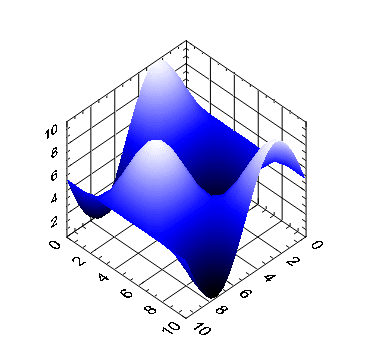
\includegraphics[scale=0.80]{example.png}
\label{img:example}
\end{figure}

Figure \ref{img:example} is just a random image I found through Google on National Instrument's website \cite{example}.

\subsubsection{How Deep Can You Go?}

This is the deepest you can go in terms of chapters and sections (i.e., you cannot go deeper than a sub-sub-section). By default, these sub-sub-sections do not appear in the table of contents, and are merely given bold headings in the document itself.

\subsection{A Long Table}

Long tables are rather confusing to use, and consist of many layers of LaTeX packaging and rendering.  Try to avoid them as best you can, but if you must use them, here is an example.  There are plenty more examples online, of course.

\begin{center}
\begin{singlespace}
\begin{longtable}[!h]{| p{5cm} | p{2cm} || p{8cm} |}
	\caption[An example programming API listing using the longtable format.]{An example programming API listing using the longtable format.}
	\label{table:long_example} \\

	\hline
		\multicolumn{1}{|c|}{Command} & 
		\multicolumn{1}{|c||}{Data} & 
		\multicolumn{1}{|c|}{Description} \\ \hline \hline
	\endfirsthead

	\multicolumn{3}{c}{{\tablename} \thetable{} -- Continued} \\
		\hline
		\multicolumn{1}{|c|}{Command} & 
		\multicolumn{1}{|c||}{Data} & 
		\multicolumn{1}{|c|}{Description} \\ \hline \hline
	\endhead

	\multicolumn{3}{|r|}{{Continued on next page\ldots}} \\ \hline 
	\endfoot

	\hline 
	\endlastfoot

	robot\_dance & dance move & Make the robot perform the specified dance move.\\ \hline
	robot\_talk & text & Make the robot speak the specified text.\\ \hline
	robot\_hug & target & The robot will seek out the specified target and give it a hug.\\ \hline
	robot\_sleep & hours & The robot will go to sleep for the specified number of hours.\\ \hline
	\end{longtable}
\end{singlespace}
\end{center}

Table \ref{table:long_example} extends through a page break, and could even be longer than one page if there was enough information in it. Note how LaTeX reprints the title/caption, and continues the formatting between pages.

\chapter{Conclusion}
\markright{Benjamin C. Hilburn \hfill Chapter 3. Conclusion \hfill}

Huzzah! You did some cool stuff and make some awesome contributions.

\section{Publication List}

It is generally customary to include a publication list in your thesis.

\begin{itemize}
	\item A publication!
	\item A second publication!
\end{itemize}


% Your bibliography will actually be rendered as a separate 'chapter' in LaTeX.  
% Thus, the Conclusion chapter ends as soon as you begin describing your 
% bibliography.  By default, the bibliography will not be included in the table 
% of contents.  This is required by the ETD, however, so we must explicitly add 
% it.  Make sure to specify your bibliography style and the path to your bibtex % file.  Remember that the path to your bibtex file does NOT include the file 
% extension.  So, in the example below, the bibtex file is in ./refs/thesis.bib, 
% and we are also referencing the system-wide IEEE abbreviation reference 
% database.
\bibliographystyle{IEEEtran}
\addcontentsline{toc}{chapter}{Bibliography}
\bibliography{IEEEabrv,./refs/thesis}

\end{document}
